%!TEX root = ../thesis.tex

%invariant enviroment
\newenvironment{invariants}{%
  \refstepcounter{thrm}%
  \paragraph{Invariants~\theprop}%
  \renewcommand*{\theenumi}{\theprop\,(I\arabic{enumi})}%
  \renewcommand*{\labelenumi}{(I\arabic{enumi})}%
  \enumerate
}{%
  \endenumerate
}

\section{Unified Algoritmh}
\fxerror[inline]{For now this chaper assumes we did not need to make moves when creating fences}

Now we have presented sweepline based algorithms that preserver vertical and horizontal onesidedness respectivly. We will now introduce an alorithm that gives a $(k,\infty)$-sided rectangular dual for any graph without seperating $4$-cycles. we will show an algoritm exists with $k=17$

\paragraph{Outline}
The approach taken by this algorithm will be the following
\begin{enumerate}
  \item Sudived the graph by fences as in the red algorithm
  \item If a blue face inbetween two fences is too long we will flip some of it's inetrior edges. We try to prevent the creation of blue Z's unless it's absolutely necessary.
  \item We solve the blue Z's we have creasted by doing a few flips.
\end{enumerate}


 \subsection{Fans and curls}
 In order to effectivly describe the algorithm and its proof we will have to introduce some more concepts.

 Consider a blue face inbetween two fences, we will call such a face a \emph{strip}. Every interior edge of this face goes from one fence to the other (due to property \ref{e:crossingEdges}). We will desribe the edges from $\spl(F)$ to $\mrg(F)$ .

 Let $u_0 , u_1, \ldots u_n$ be the vertices of the upper boundary path of $F$ and $v_0, v_1, \ldots, v_m$ the vertices of the bottom boundary path. That is $u_0=v_0 = \spl(F)$ and $u_n = v_m = \mrg(F)$. Since our graph is a triangulation $u_1v_1$ must be an edge. For the second edge in the face we have two options $u_1v_2$ or $u_2v_1$, otherwise this edge and the previous one would not form a traingle. This principle holds for every subsequent edge, we can either increase a the index of the upper boundary path or the index of the bottom boundary path.

 We will call a maximal series of at least two edges increasing the index on the bottom boundary path (and thus keeping the index on the upper path fixed) a \emph{fan} and a maximal series of at lest two edges increasing the index on the upper boundary path will be called a \emph{curl}. The \emph{size} of such a fan or curl is the number of edges contained in the series. By the definition of fan and curl each fan or curl has size at least $2$.

 In Figure \ref{fig:uni:fansandcurls} we see a strip consisting of subsequently a curl of size $2$, a fan of size 2, a curl of size $2$, a fan of size $6$, a curl of size $3$ and a fan of size $3$.

 \begin{figure}[h]
   \centering
   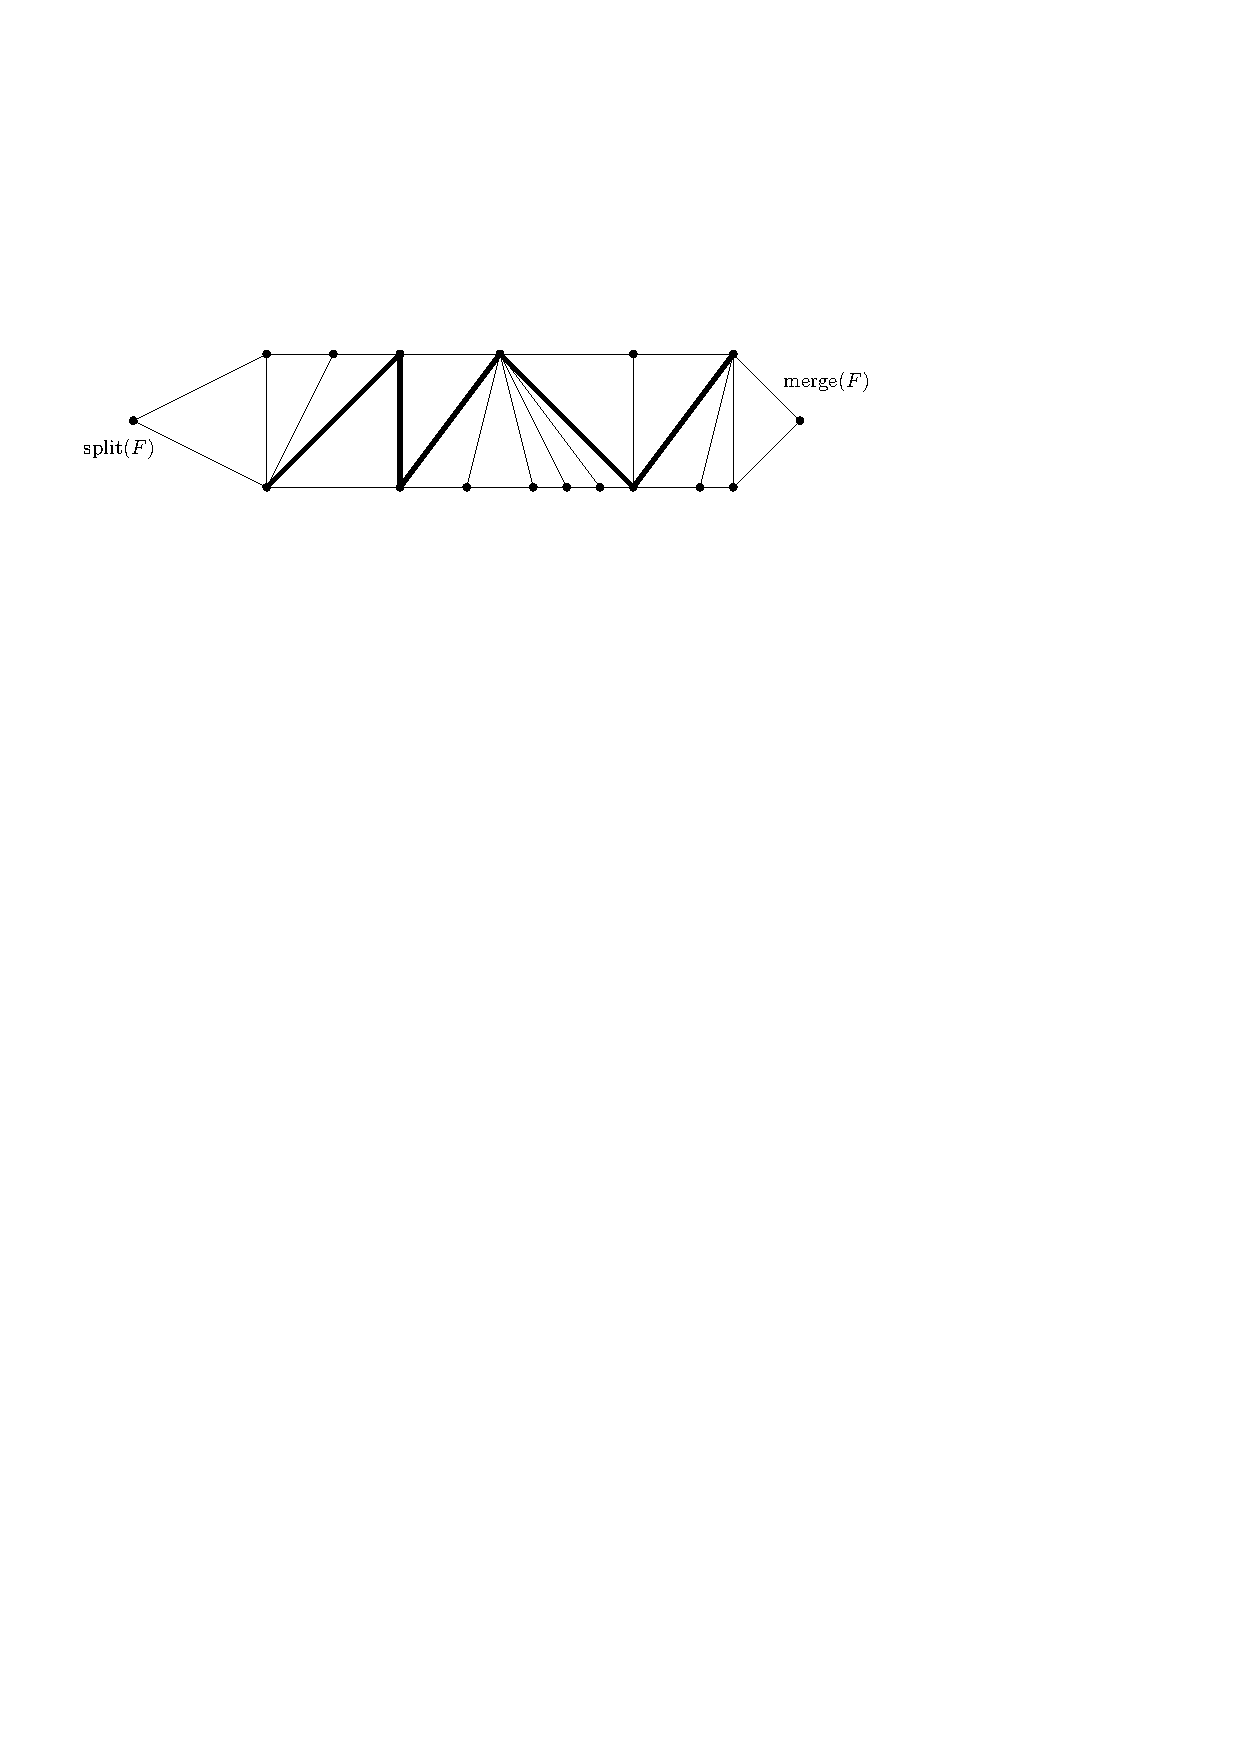
\includegraphics[scale=.9]{unifiedAlgo/img/fansandcurls}
   \caption{}
   \label{fig:uni:fansandcurls}
 \end{figure}


In a strip we alternately encounter curls and fans. Since suppose we would have two adjacent fans or curls then we would just have a larger fan or curl.

We will sometimes shorten our notation and let for example $c3$ mean a curl of size $3$ and $f2$ a fan of size $2$. Then in this notation the strip in Figure \ref{fig:uni:fansandcurls} can be characterized by $c2 f2 c2 f5 c3 f3$. In this \emph{short notation} of a strip we will sometimes use notation to express we have a large  or small curl without giving it's size explicitly. We will take $c4-$ mean a curl of size $4$ or less and $c3+$ a curl of size $3$ or larger.  Furthermore $c?$ is a curl of any size and $c\infty$ is an infinitively large curl.
\footnote{this is useful in counterexamples.} A large curl can thus be expressed as $c5+$

Note that the only edges that are flippable are those that are in both a fan and a curl.
\fxnote{We might want to show this}


We introduce some more terminology for curls \emph{outer edges} and \emph{pads}
 \fxwarning{TODO}
\begin{figure}[h]
  \centering
  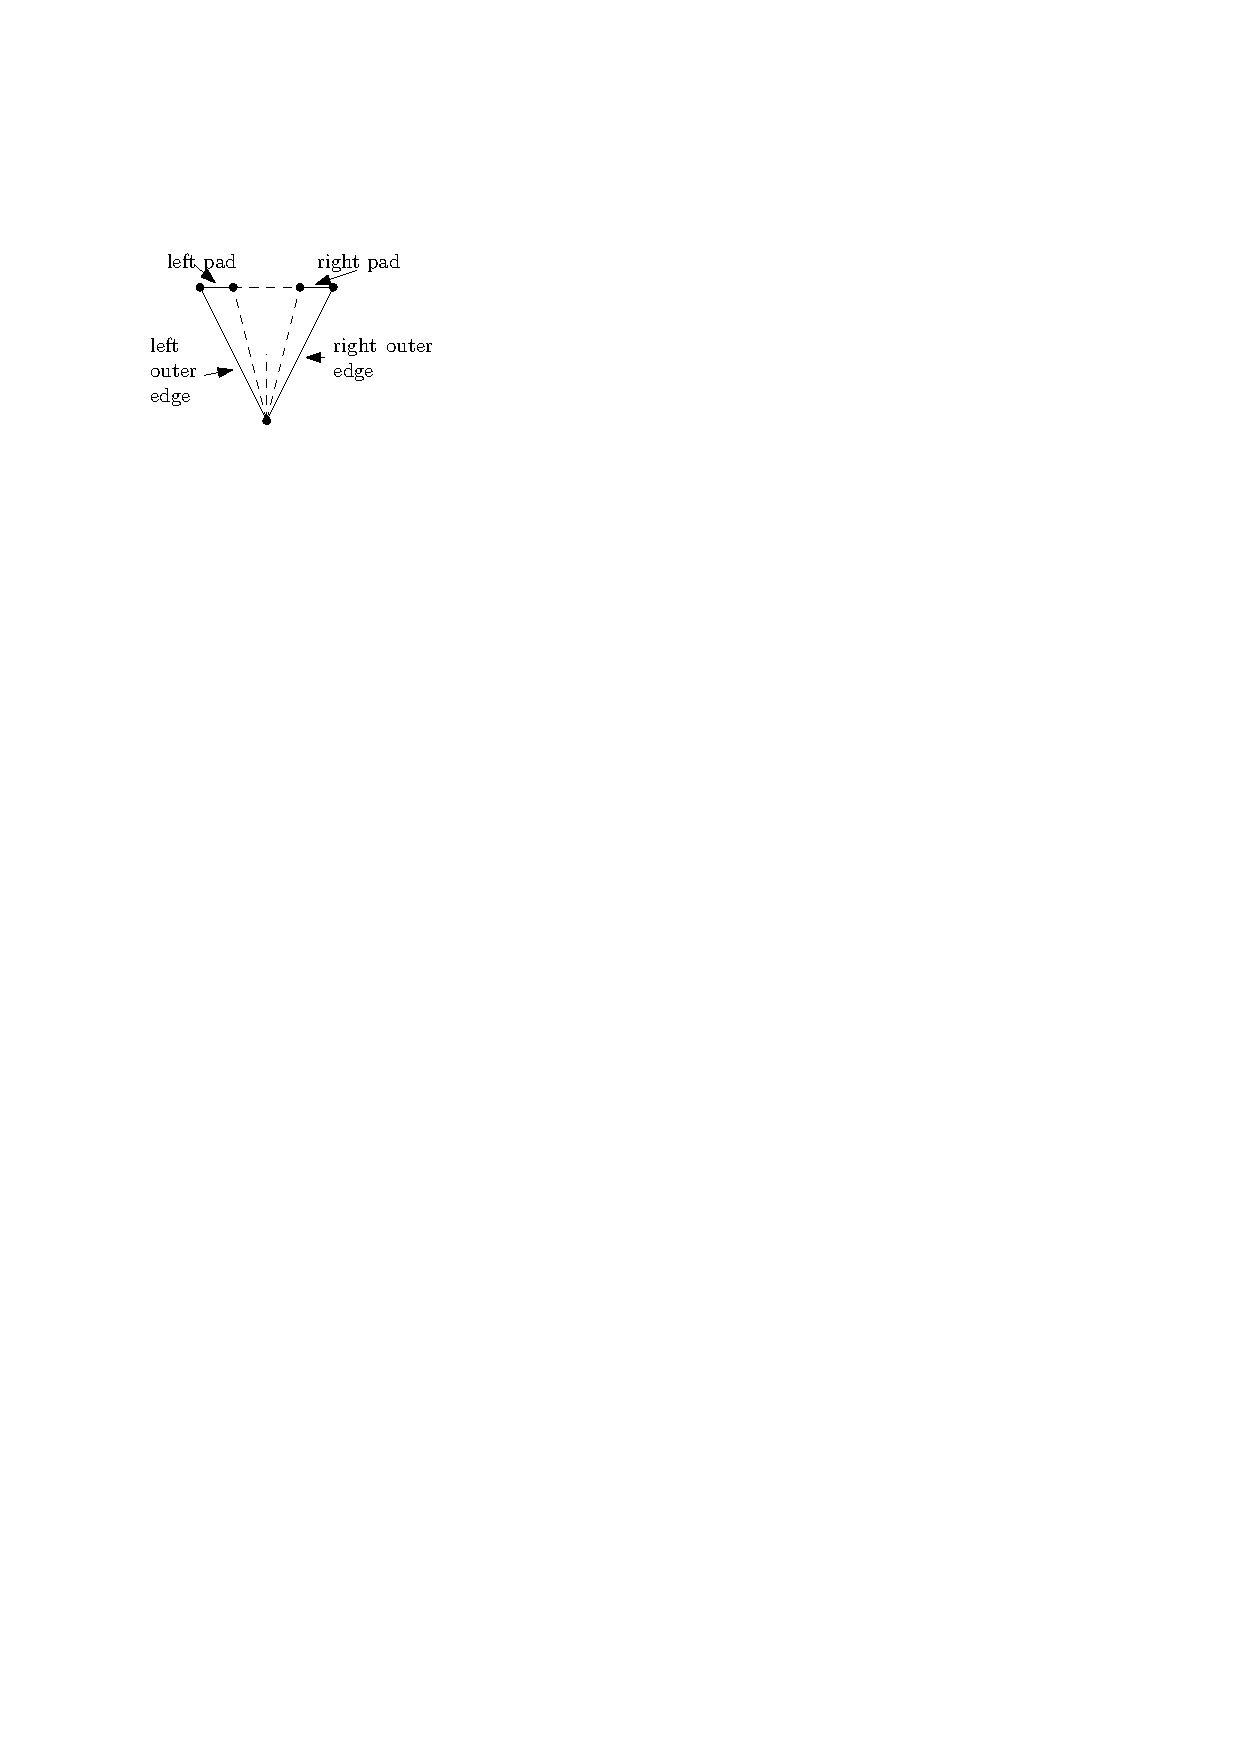
\includegraphics[scale=1]{unifiedAlgo/img/curlterms}
  \caption{}
  \label{fig:}
\end{figure}


\subsection{Preliminary results}

\begin{lemma}
  \label{lm:}
  A graph without overlapping blue $Z$'s is vertically $(2, \infty)$ sided.
\end{lemma}
This depends how we define overlap, it seems true for vertex overlap

\begin{lemma}
  \label{lm:}
  Above curl we have fans of size $2$
\end{lemma}
\begin{proof}
  Otherwise we create a $4$-cycle
\end{proof}


\subsection{Algorithm}
There is a partial order of strips. we start with the largest element and can always treat such a strip such that all strips larger than that strip are already treated while all strips smaller than that strip are note yet treated.
 \fxwarning{TODO Does this order exists, find ref in literature}

\paragraph{Loaded edges}
While doing flips we want to prevent the creation of multiple connected blue Z's, since these can lead to very large red faces. In order to prevent this we will introduce the concept of a \emph{loaded} edge on a fence. Every time we flip an edge and thus create a blue $Z$ we mark the bottommost edge of this $Z$ as loaded. During the rest of the algorithm we will be very careful in using loaded edges in our flips.

\begin{figure}[h]
  \centering
  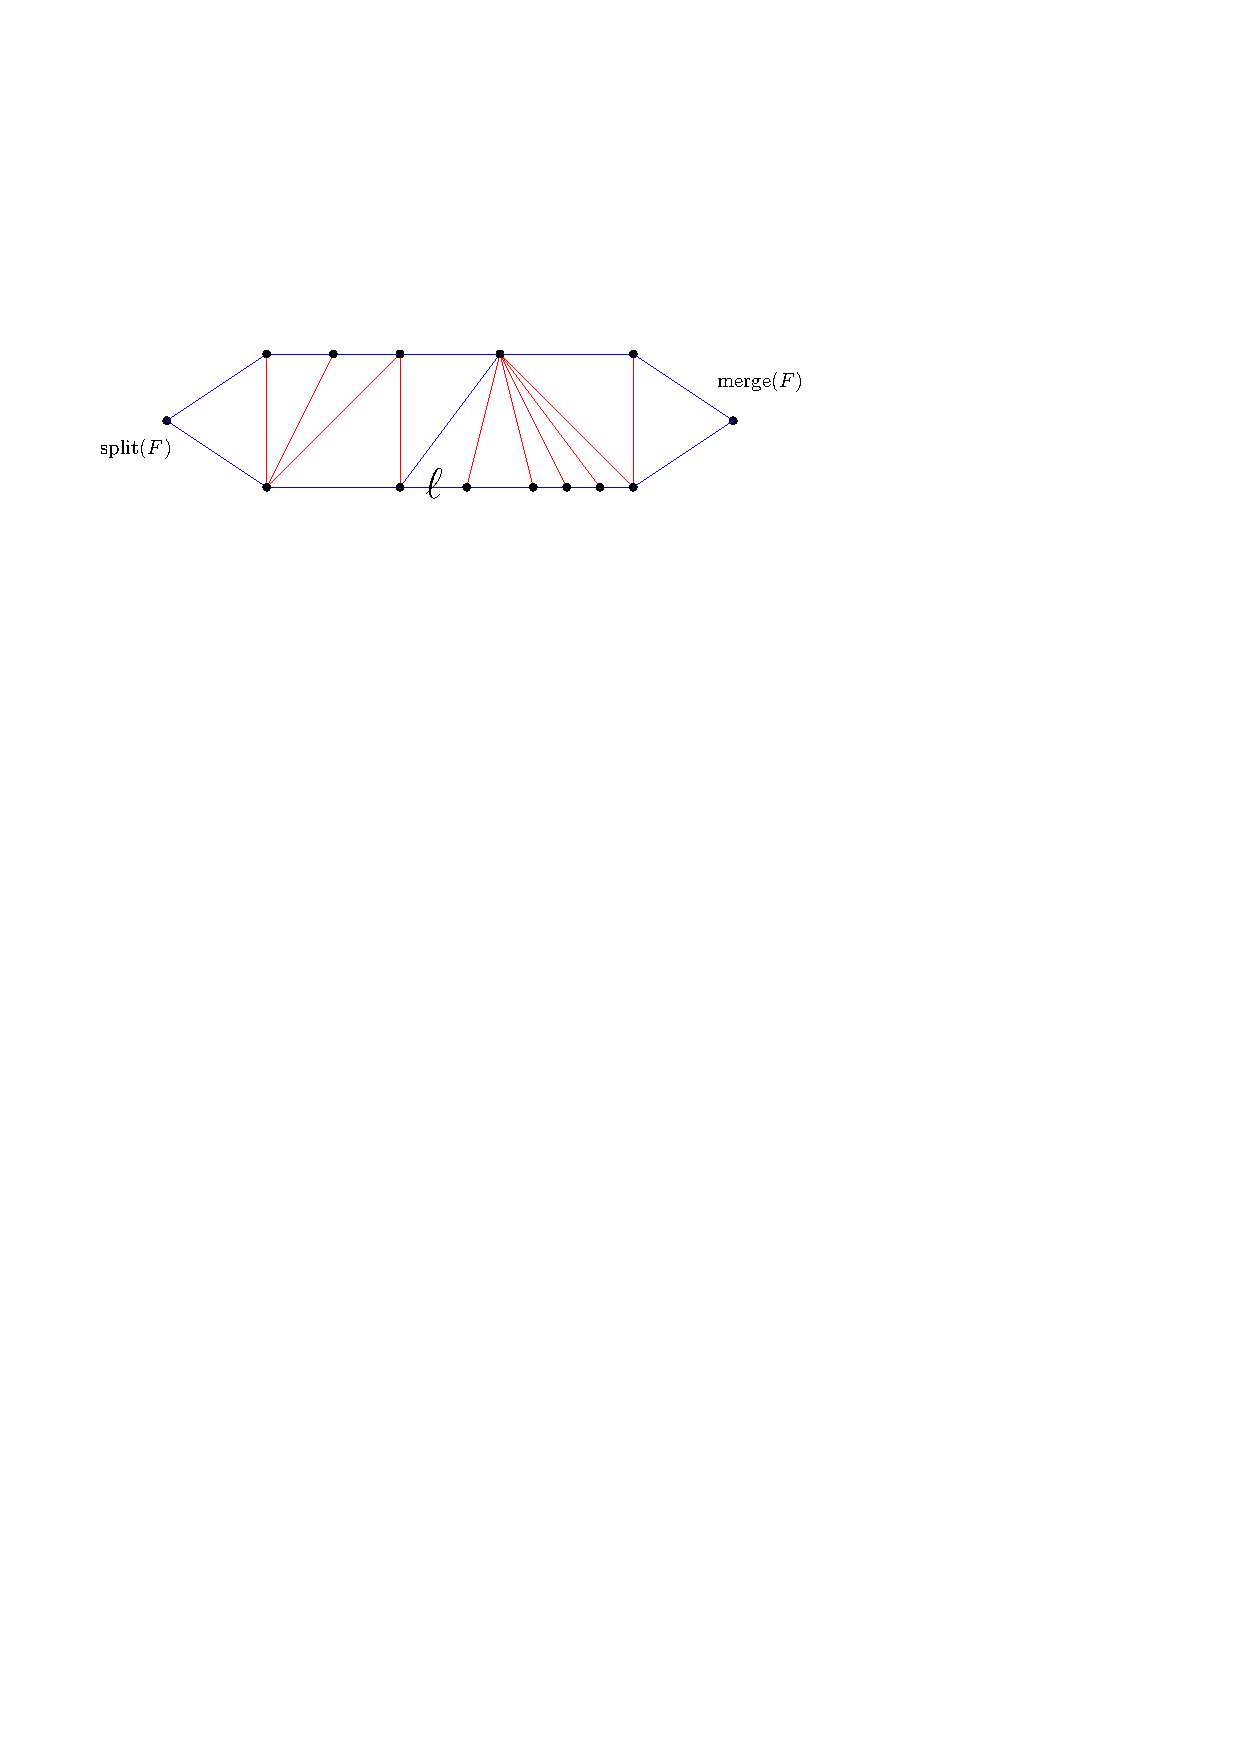
\includegraphics[scale=1]{unifiedAlgo/img/load}
  \caption{The algorithm has decided to flip an edge. The bottommost edge of the freshly formed edge is marked as being loaded. }
  \label{fig:uni:load}
\end{figure}

\subsubsection{Treating a strip}
\newcounter{invar}
While deciding which edges to flip on each strip we will maintain the following invariants

\begin{invariants}
  \label{inv:uni:load}
  \item The loaded edges on the next fence occur in one of the following patterns: 1 loaded edge followed by at least 1 unloaded edge, 2 loaded edges followed by at least two unloaded edges.

  \setcounter{invar}{1}
\end{invariants}

\paragraph{Removing large curls}

For each strip we first flip both outer edges of any curl of size $5$ or larger. Such a curl will be called a \emph{large curl}.

We will show that we can create blue faces that are at most $(9, \infty)$ containing all the large curls and obeying Invariant \ref{inv:uni:load}.

\begin{lemma}
  \label{lm:}
  We can create blue faces that are at most $(9, \infty)$ containing all the large curls and obeying Invariant \ref{inv:uni:load}.
\end{lemma}


\begin{proof}
  we will begin scanning at the split of the strip when we encounter a large curl ($c5+$) we  will enter a multistage case distinction ending with a small enough blue face and and edges on the bottom fence of the strip satisfying Invariant \ref{inv:uni:load}.

  Note that in all cases we flip the left outer edge of the first $c5+$ we encounter when scanning. Also note that we only ever flip edges bordering a large curl.


  Let us first inspect the 3 fans following our $c5+$. If any of them is size 5 or larger we flip the right outer edge of the last large curl before this fan and continue our scan from the fan onward. In this case the largest face we create is $(7, \infty)$.

  Otherwise all three fans following our $c5+$ are small, we have the following sequence $c5+ f4- c? f4- c? f4- c?$. If the rightmost curl is large we continue our scan at this curl, creating a $(9, \infty)$- face. Otherwise, if the second-right most curl is large we continue our scan there creating a $(6, \infty)$-face.

  Otherwise we check whether the third-rightmost curl is large if this is the case we flip it's \textbf{right} outer edge and continue our scan after this curl. Otherwise we also flip the \textbf{right} outer edge of the original $c5+$. We continue the scan right after this flipped edge. In both cases we can do this without offending Invariant \ref{inv:uni:load} since the next two/three curls are small so the next one/two edges will not be loaded even when continuing the scan immediately after. These last two steps yield faces of size at most $(4, \infty)$.

  One can also see the order in which we try to place edges in Figure \ref{fig:uni:placeedges}

  \begin{figure}[h]
    \centering
    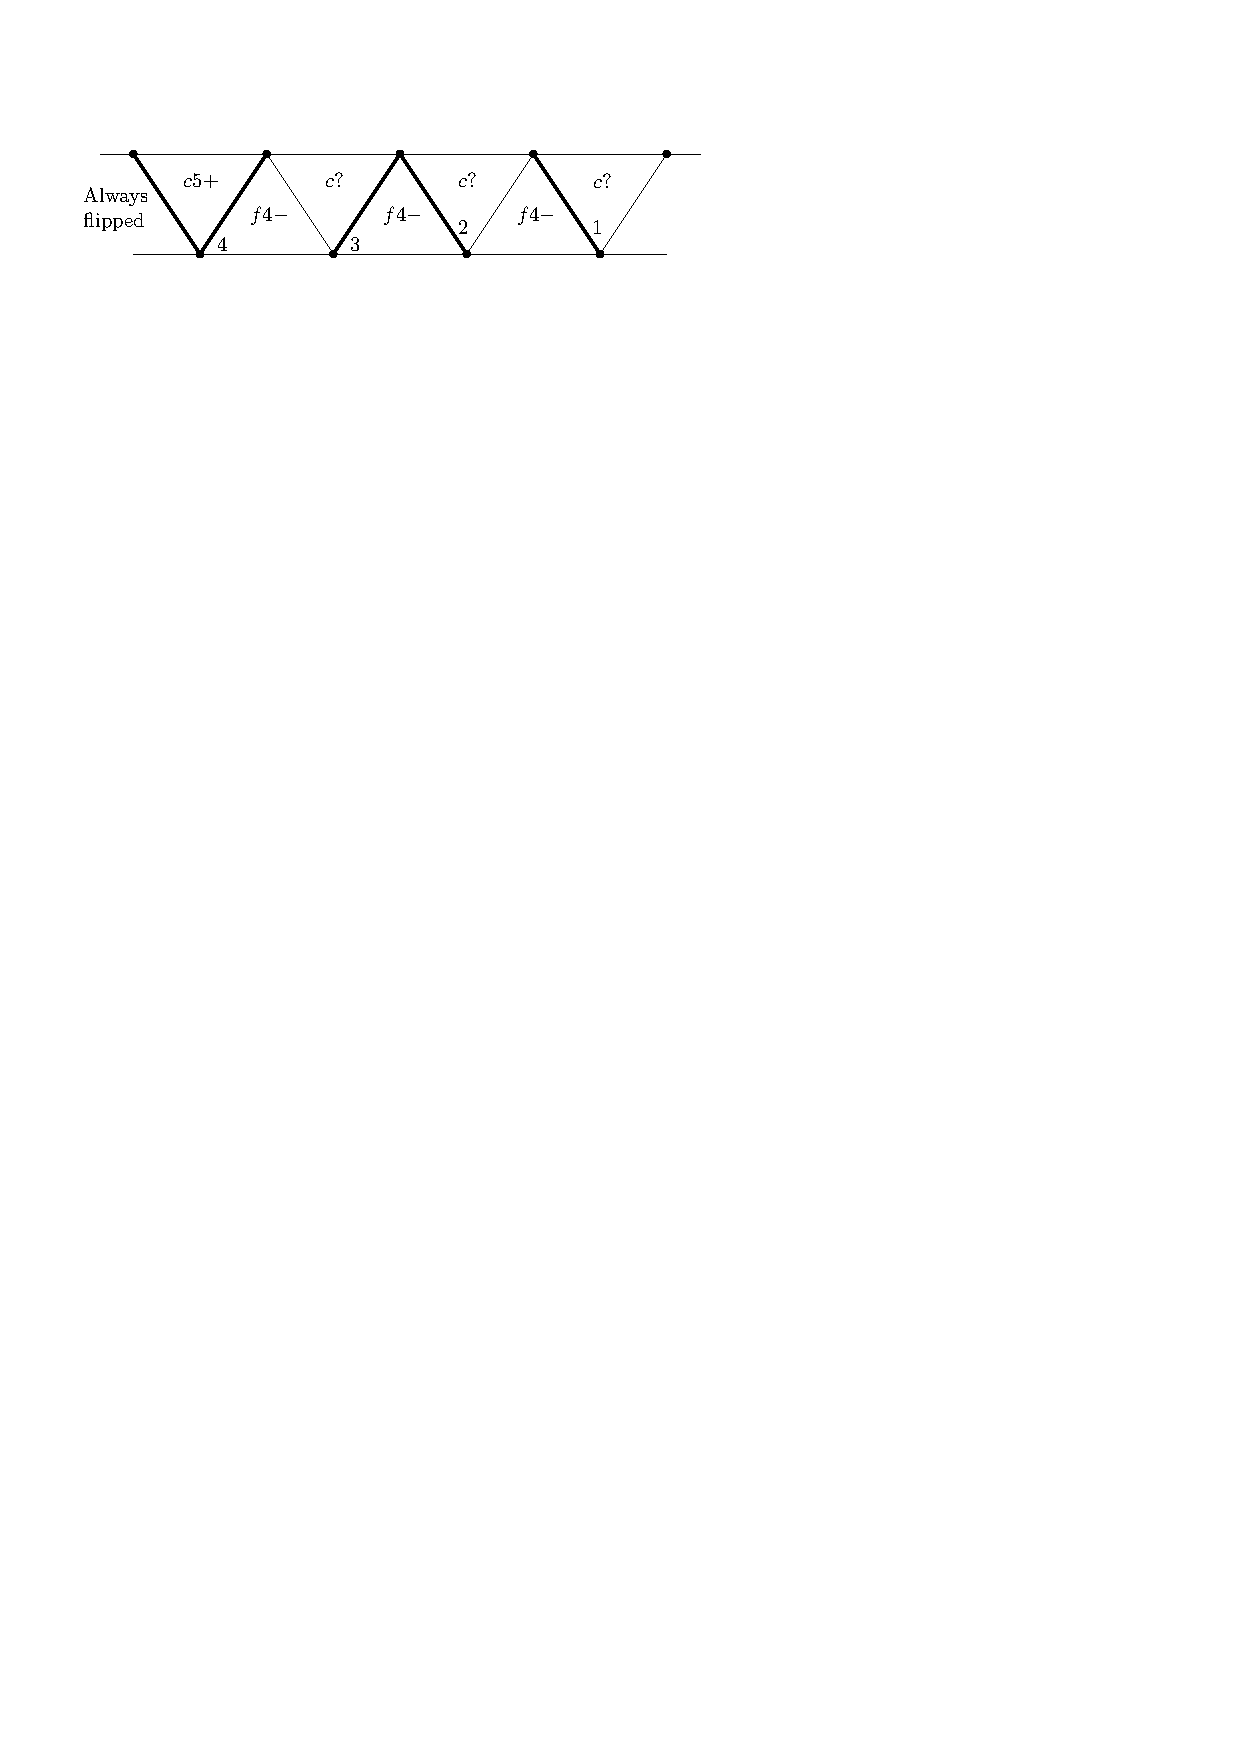
\includegraphics[scale=1]{unifiedAlgo/img/placeEdges}
    \caption{Order in which we try to flip edges. We only flip an edge if it neighbors a large curl.}
    \label{fig:uni:placeedges}
  \end{figure}

\end{proof}

  Note that we only ever flipped outer edges of a $c5+$ in this proof


\paragraph{The rest of the strip}

Any further blue faces that are still to large do not contain any large curls. We will be careful to flip only if we satisfy the following invariants in addition to Invariants \ref{inv:uni:load}

\begin{invariants}
  \label{inv:uni:rest}
  \item We don't flip an edge creating a blue $Z$ containing a loaded edge.
  \item We don't flip an edge creating a blue $Z$ containing a pad of a large curl in the next strip.
\end{invariants}

 \fxwarning{TODO give these a proper ref and environment (beore starting real proofs)}

We consider two cases for our still to large blue face $F$, either this blue face is above the entirety of a large curl in the next strip or it isn't.
In the first case we can find a flippable edge satisfying all the invariants and we are done.

\begin{lemma}
  \label{lm:uni:flipAboveLargeCurl}
  We can flip at least one edge above in any blue face that lies above the entirety of a large curl in the next strip.
  \fxnote{This lemma should probably change when we start to allow moves}
\end{lemma}
\begin{proof}
  In the strip above a large curl and directly above such a large curl any fan can only be of size $2$ since otherwise we would have a separating $4$-cycle \fxnote{I could/should make this a lemma somewhere}. Furthermore there can't be large curl in the face we are treating since all large curls are in $(9,\infty)$ faces.  We are thus in the situation depicted in Figure \ref{fig:uni:flipAboveLargeCurl}.

  \begin{figure}[h]
    \centering
    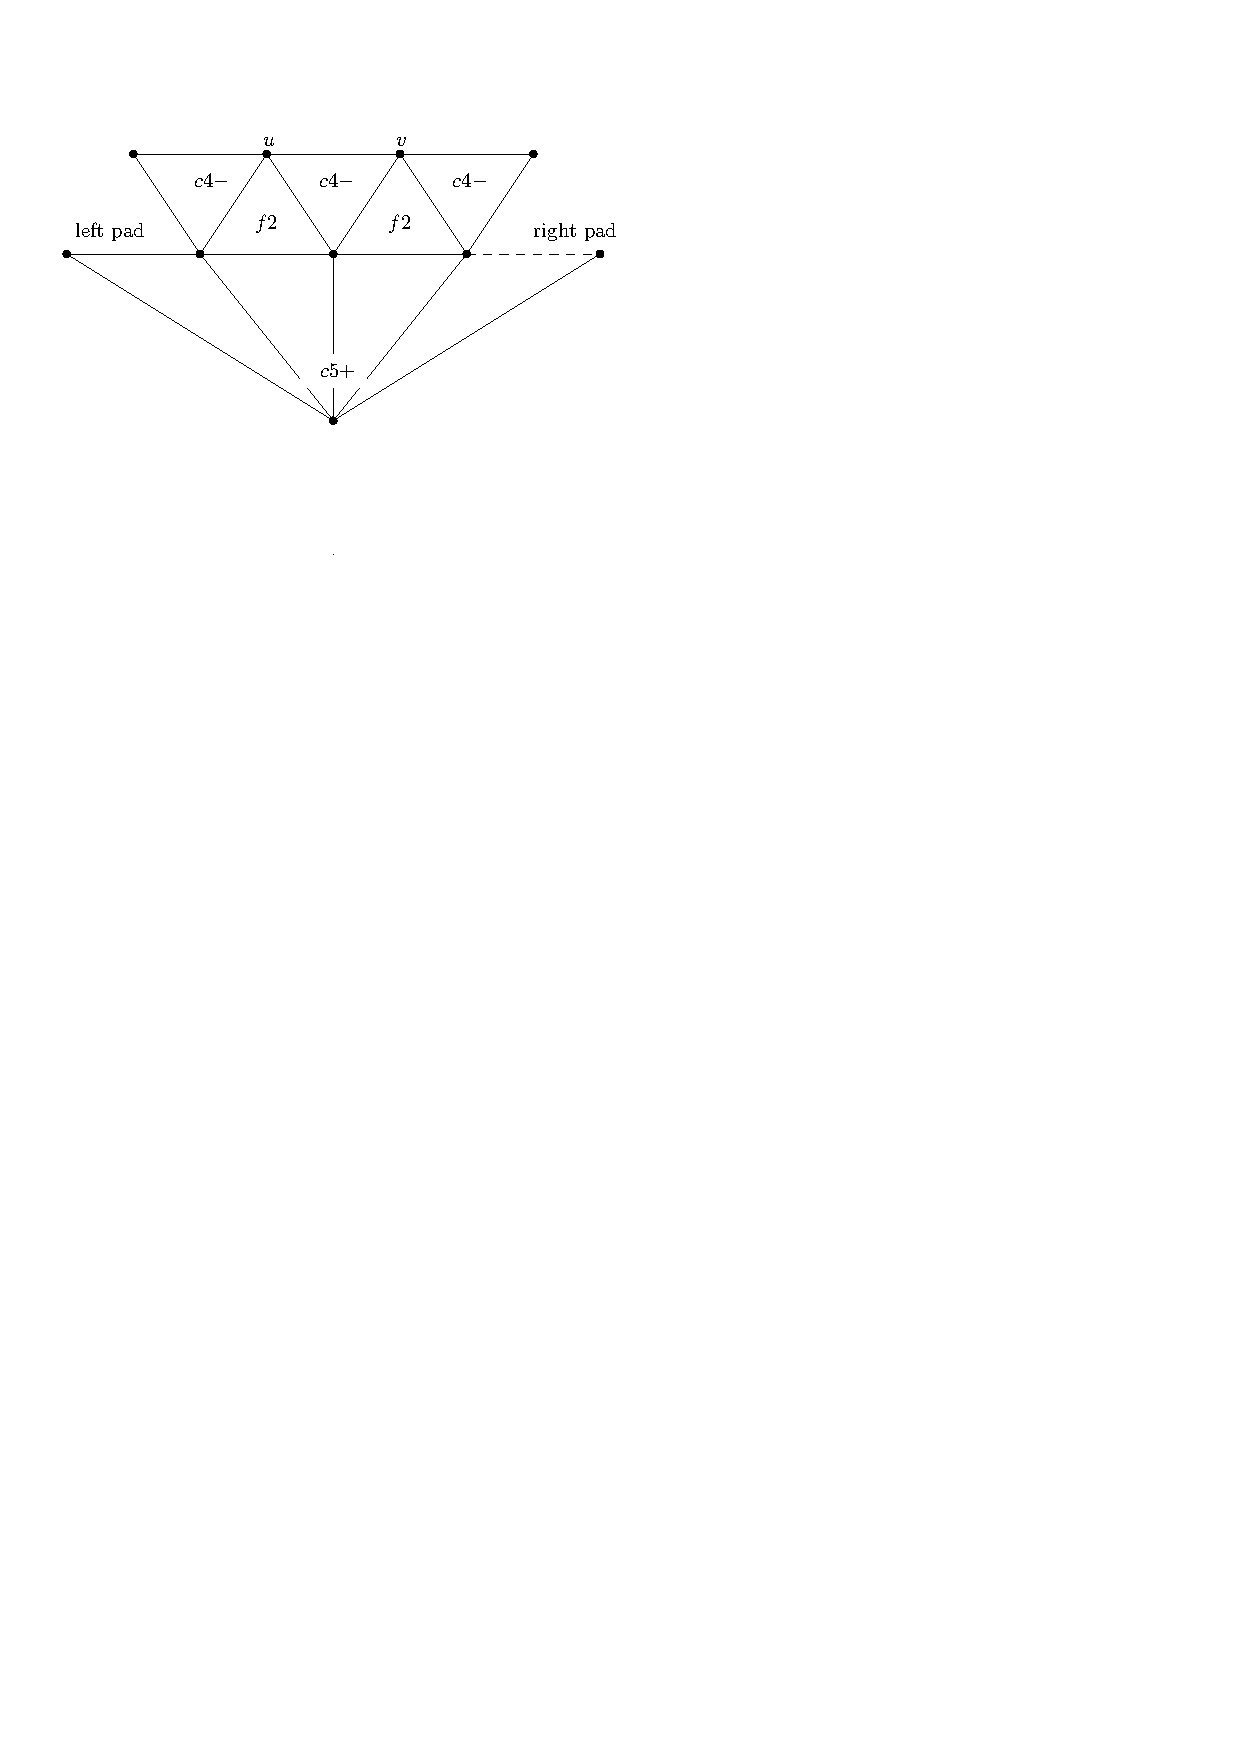
\includegraphics[scale=1]{unifiedAlgo/img/flipAboveLargeCurl}
    \caption{}
    \label{fig:uni:flipAboveLargeCurl}
  \end{figure}

  Now suppose one of the edges neighboring $u$ is not loaded then we can flip here. Now let us assume both edges incident to $u$ on the fence are loaded then at least one of the edges of the fence incident to $v$ is unloadned  because the next two edges are unloaded due to Invariant \ref{inv:uni:load}.

  Hence we can alway flip an edge above a large curl.
\end{proof}


In the second case we don't have to consider more then one right pad and more the one left pad otherwise we could execute Lemma \ref{lm:uni:flipAboveLargeCurl}

\begin{lemma}
  \label{lm:}
  In any blue face that is not a $(25, \infty)$ blue face  we can flip a edge.
\end{lemma}
\begin{proof}
  The face under consideration does not lie above the enirty of any curl becuase of Lemma \ref{lm:uni:flipAboveLargeCurl}.

  Such a face that is not $(31, \infty)$ has at least $32$ vertices on the top fence. This means it has at least $31$ edges lying in at least $11$ curls. These curls have $10$ inbetween fans. The two fans  closest to the both border of the face will remain unloaded in order to preserve Invariant \ref{inv:uni:load}. This leaves $6$ fans. One pad or two loaded edges can pssibly block an entire fan. We can't block two subsequent fans with loaded edges due to only small curls. We only have two pads. So one of the fans has to remain free and we can thus flip an edge satisfying both Invariants \ref{inv:uni:load} and \ref{inv:uni:rest}.
\end{proof}


\paragraph{Flips}
After we have treated all strips the only overlapping blue $Z$'s are those that have their middle  edge (the one crossing a strip) as outer edge of a large curl. This because the rest of the edges has been placed obeying the properties above.


We only treat long sequences of adjacent $Z$'s  because otherwise we don't necessarily improve things.


We can then have essentially two cases
 \fxwarning{TODO argue this}
who are depicted in Figure \ref{fig:uni:flipcases} we treat these as depicted in Figure \ref{fig:uni:flipaction}.


\begin{figure}[h]
  \centering
  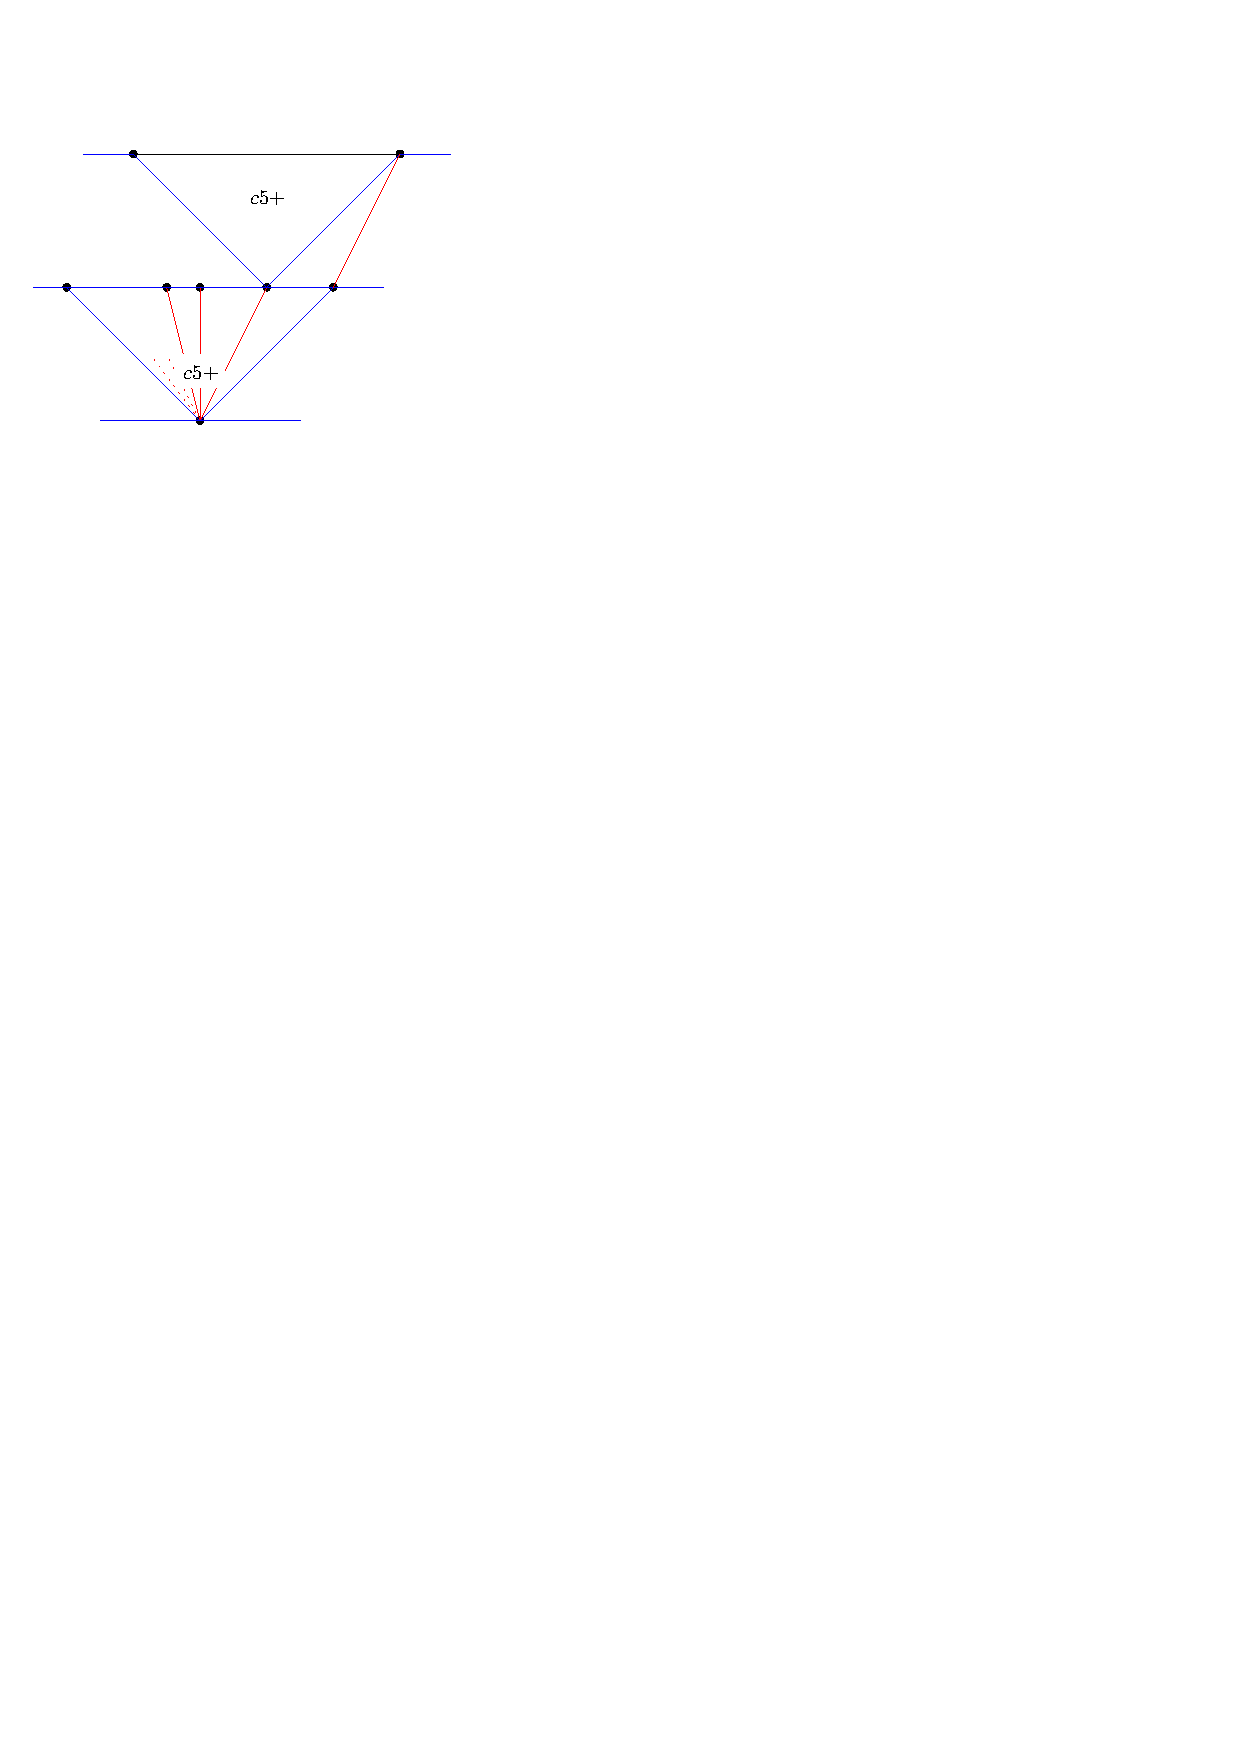
\includegraphics[scale=1]{unifiedAlgo/img/flipcasea}
  \caption{Case a) before the flip}
  \label{fig:uni:flipcasea}
\end{figure}

\begin{figure}[h]
  \centering
  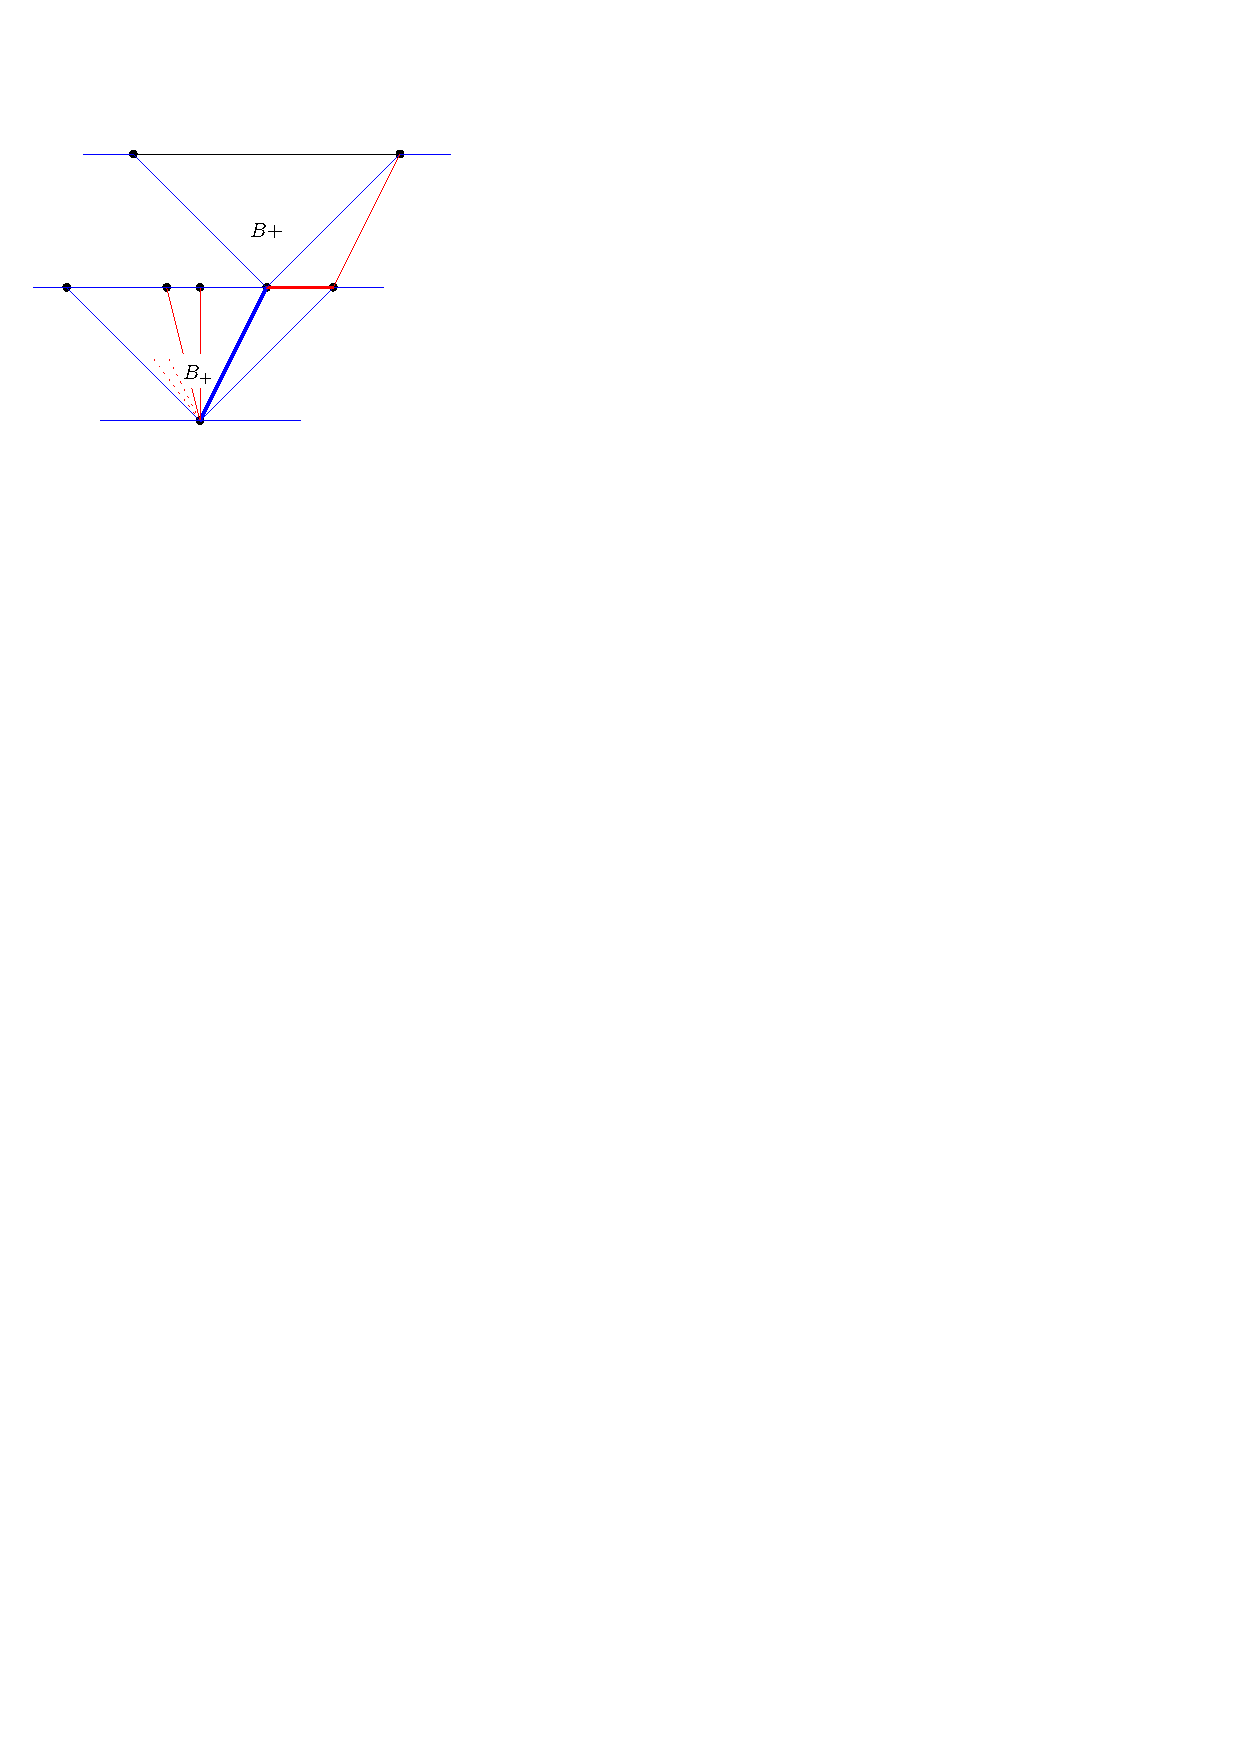
\includegraphics[scale=1]{unifiedAlgo/img/flipactiona}
  \caption{Case a) after the flip}
  \label{fig:uni:flipactiona}
\end{figure}

\begin{figure}[h]
  \centering
  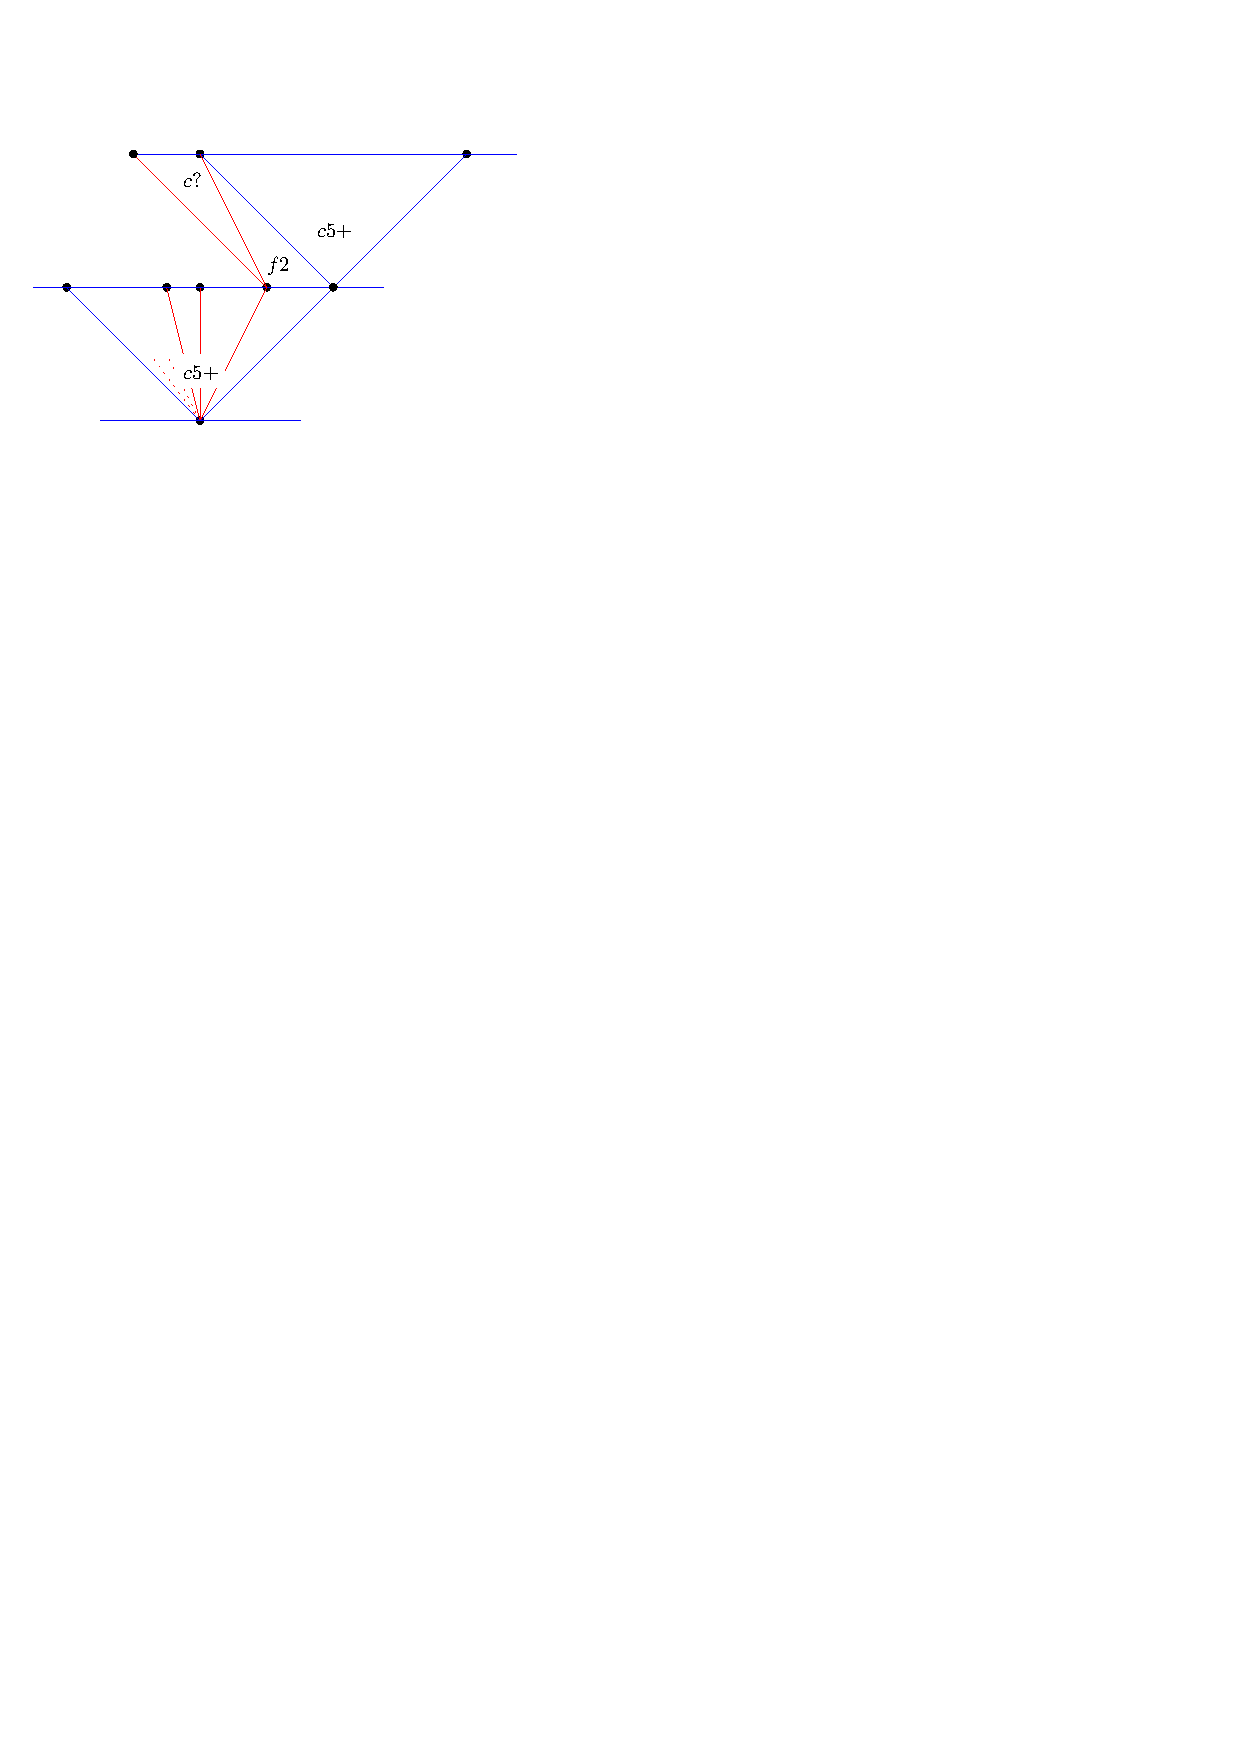
\includegraphics[scale=1]{unifiedAlgo/img/flipcaseb}
  \caption{Case b) before the flip}
  \label{fig:uni:flipcaseb}
\end{figure}

\begin{figure}[h]
  \centering
  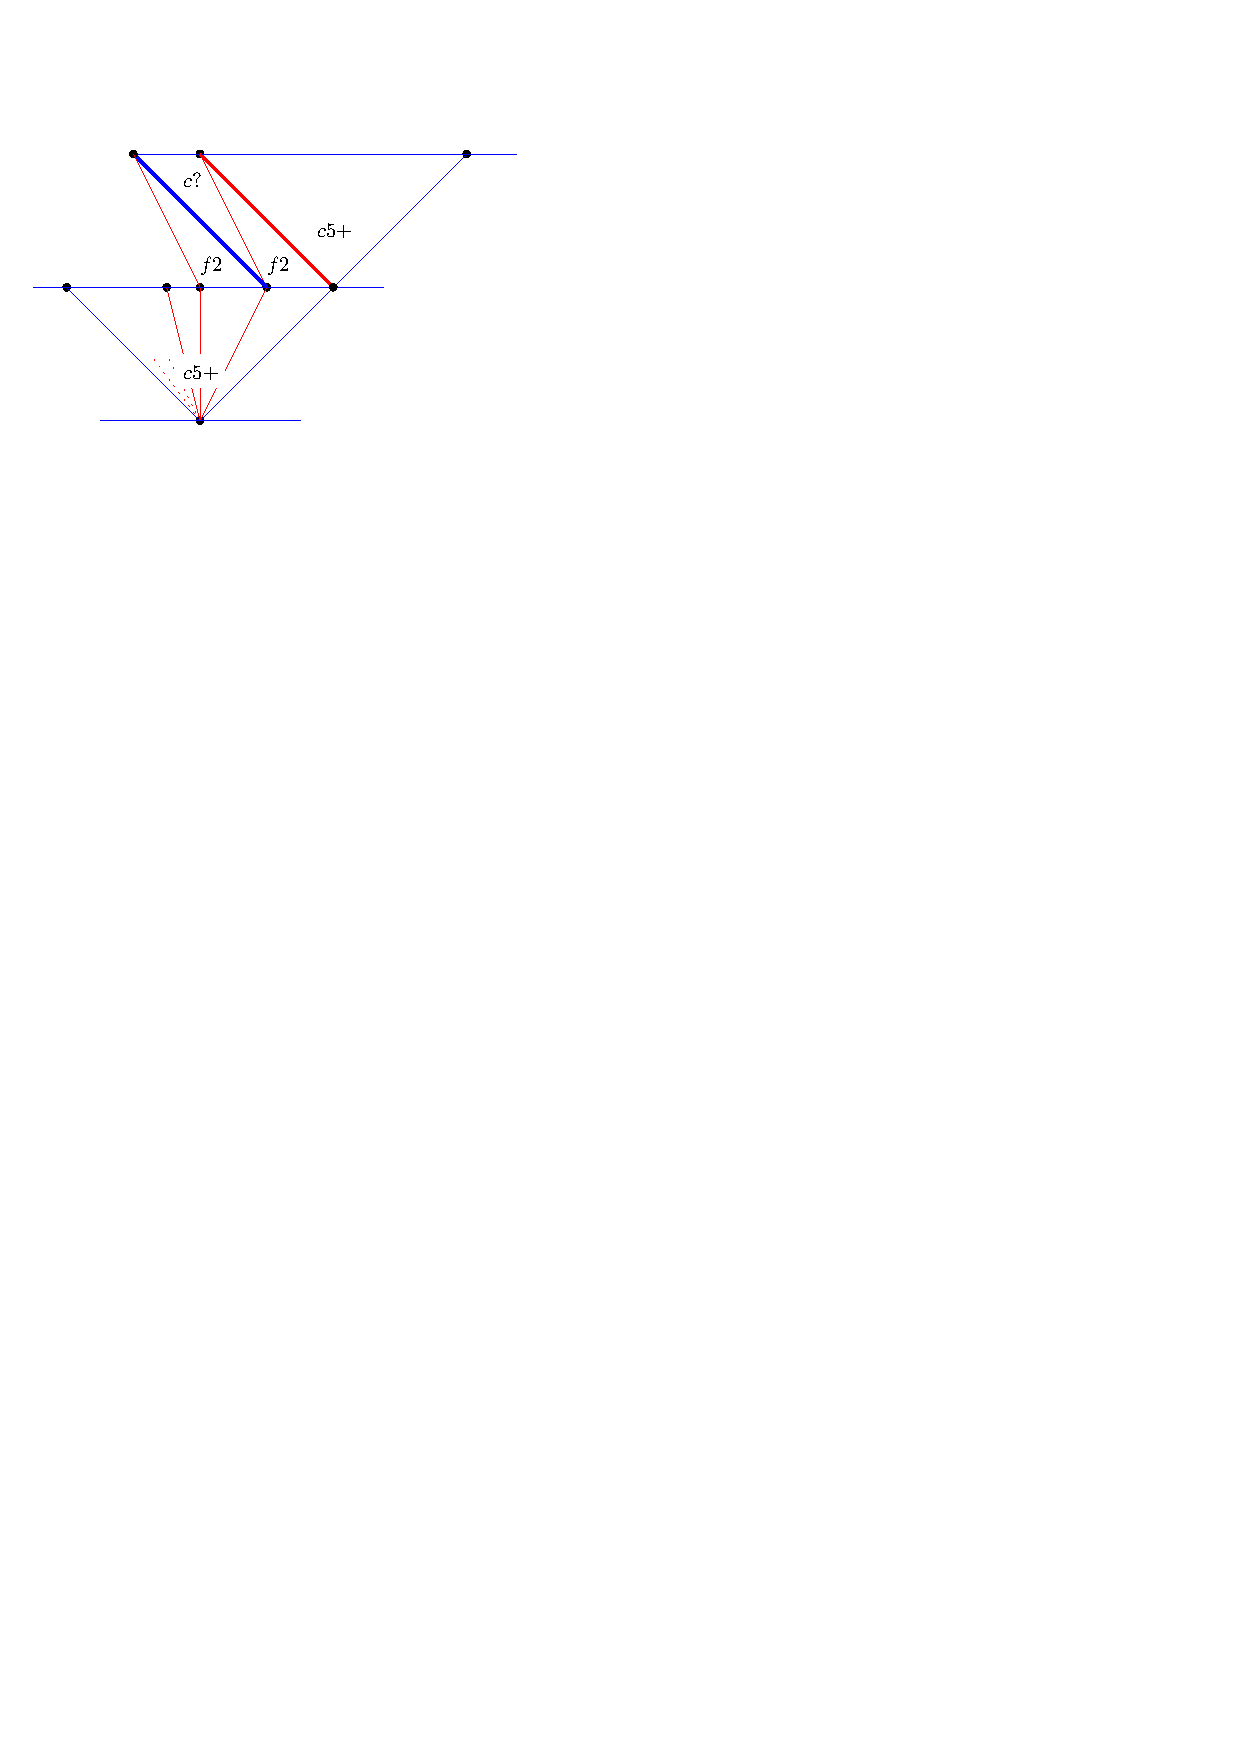
\includegraphics[scale=1]{unifiedAlgo/img/flipactionb}
  \caption{Case b) after the flip}
  \label{fig:uni:flipactionb}
\end{figure}

\subsection{Correctness}
